\documentclass[../main.tex]{subfiles}
\graphicspath{{\subfix{../images/}}}

\begin{document}

\hypertarget{opencrs}{%
  \chapter{OpenCRS}\label{opencrs}}

This study, together with Claudiu Ghenea's \cite{ghenea}, presents an
open-source cyber reasoning system. OpenCRS aims to implement a comprehensive
security assessment process for executables by utilizing the latest
advancements in binary analysis from both academic and industrial sectors. The
purpose of OpenCRS is to execute a comprehensive security evaluation of
executable files, encompassing the identification of input methods and the
development of patches to address any detected vulnerabilities.

Given the significant diversity in architectures, programming languages, and
binary behaviors, the objective was to create a proof of concept that addresses
the execution of programs exhibiting the subsequent attributes:

\begin{itemize}
  \tightlist
  \item
        The system operates on a 32-bit Intel architecture, specifically
        utilizing the \texttt{i386} instruction set architecture.
  \item
        The software is compatible with the Linux operating system and
        utilizes the ELF format.
  \item
        These are generated from the source code written in the C programming
        language.
  \item
        The input streams for arguments, standard input, and files are
        utilized.
\end{itemize}

The diagram below depicts the comprehensive architecture of OpenCRS and the
inter-module communication taking place within the system.

\begin{landscape}
  \renewcommand*\figurename{Figure}
  \begin{figure}[!h]
    \centering
    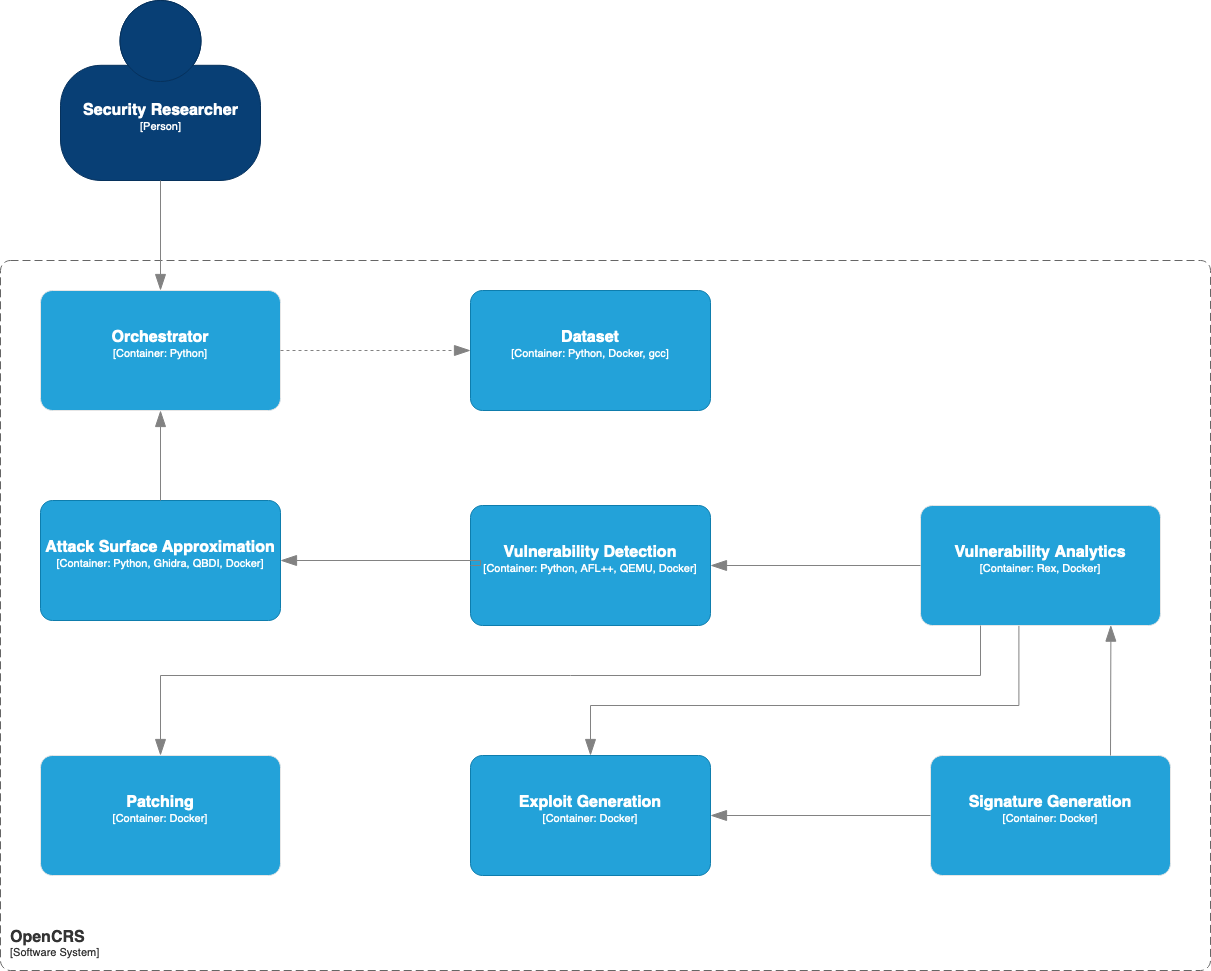
\includegraphics[height=0.95\textheight]{images/opencrs.png}
    \caption{OpenCRS's Architecture}
    \label{fig:opencrs_architecture}
  \end{figure}
\end{landscape}

Given that an analyst demands an executable analysis, the orchestration module
manages the modules and their internal procedures as follows:

\begin{enumerate}
  \def\labelenumi{\arabic{enumi}.}
  \tightlist
  \item
        Dataset module: By incorporating various public test suites into the C
        source code, the module can compile it and generate a sequence of
        executable files. The primary benefit of this methodology is that
        OpenCRS can implement a validation mechanism that takes into account
        the vulnerabilities present in the source code, as indicated by the
        CWE labels, as well as those that have been identified, exploited, and
        remediated by the system. The dataset module is not mandatory since
        the analyzed executables utilized by OpenCRS may have already been
        constructed from alternative origins. Both open-source software, such
        as HiColor\simplefootnote{https://github.com/dbohdan/hicolor}, and closed-source software, such as Dropbox\simplefootnote{https://dropbox.com}, offer their
        users the option to download prebuilt binaries that cater to a variety
        of architectures.
  \item
        Attack surface approximation module: With an executable (and no other
        knowledge about it) as input, this module will determine how it might
        be attacked: either through input streams or a predefined format for
        them (for example, the arguments that the program expects in
        \texttt{argv}).
  \item
        Vulnerability discovery module: Subsequent to the identification of
        the attack surface by the preceding module, this module will employ
        vulnerability discovery methodologies such as fuzzing and symbolic
        execution to ascertain the existence of vulnerabilities, specifically
        inputs that result in erroneous program behavior.
  \item
        Vulnerability analytics module: Upon detecting a proof of
        vulnerability, this module conducts an analysis to provide additional
        information regarding the specific vulnerability that has been
        identified. This may include identifying the category of
        vulnerability, such as a buffer overflow.
  \item
        Automatic exploit generation module: The preceding module's proof of
        vulnerability is utilized to develop an exploit that triggers it and
        has the greatest possible impact.
  \item
        Signature generation module: In contrast to the offensive nature
        of its predecessor, the module responsible for generating signatures
        serves a protective function. By utilizing identical input as the
        automatic exploit generation module, a signature is generated with the
        purpose of identifying and preventing exploitation endeavors. The
        module is deemed valuable in scenarios involving critical or outdated
        systems, wherein the installation of an alternative program is not
        feasible due to the unavailability of the program or compatibility
        issues.
  \item
        Healing module: The objective of this module is akin to that of the
        signature generation module, which is to safeguard the binary from
        exploitation techniques. In contrast to the preceding module, the
        current one has made alterations to the binary in order to eliminate
        the vulnerable code or implement appropriate sanitization measures,
        while preserving the original functionality.
\end{enumerate}

Subsequent chapters will provide a comprehensive account of the internal
operations of various modules. It is noteworthy that the outstanding modules
have been addressed in separate theses: the vulnerability analytics and healing
modules in \cite{ghenea}, and the signature generation module in \cite{stefan}.

\end{document}